%% Cache-Derived Receive Buffers for UDP
%% USENIX NSDI submission format (usenix2019_v3.sty), body only, 12 pages.
\documentclass[letterpaper,twocolumn,10pt]{article}
\usepackage{usenix2019_v3}
\usepackage{graphicx}
\usepackage{booktabs}
\usepackage{amsmath}
\usepackage{url}
\usepackage{xspace}

\newcommand{\sys}{\textsc{Weir}\xspace}
\newcommand{\rmemmax}{\texttt{rmem\_max}\xspace}
\newcommand{\rcvbuf}{\texttt{sk\_rcvbuf}\xspace}
\newcommand{\rxframes}{\texttt{rx-frames}\xspace}

\begin{document}

\title{\Large \bf Cap It From the Cache, Drop It at the Driver:\\
Rethinking the UDP Receive Buffer}

\author{}
\date{}
\maketitle

\begin{abstract}
A UDP receiver's throughput is decided by a number nobody is in a position to
set. The socket buffer must hold what one interrupt-moderation window delivers,
but the moderation frame count is chosen by the driver at run time and is
invisible to the application; the buffer must also fit, together with the NIC's
descriptor pages and every other socket's buffered data, inside the last-level
cache, a total no single socket can see. On one receiving core at 56\,Gbps, a
1\,MB buffer drops 37\% of a single flow because it cannot hold one moderation
window, and eight 8\,MB buffers lose 58\% of an eight-flow workload because
together they are three times the cache.

The natural response is to size the buffer adaptively, and we built that: the
same rule TCP uses, with the interval between the receive queue filling and
emptying standing in for the RTT. It works, and it is not the right answer. A
\emph{fixed} 1\,MB buffer with a short discard window in the driver matches it
on both workloads and beats it by 4--6\% once the core saturates, because past
that point a larger buffer only means more data evicted before the consumer
reaches it.

What the sizing experiment does establish is what a cap is for. Discarding
cannot rescue an over-large buffer---eight 8\,MB sockets reach 29.4\,Gbps with
discarding against 22.7 without, and 55.8 with a 1\,MB buffer---because removing
work does not remove capacity, and capacity is what thrashes the cache. We
therefore propose two mechanisms and no controller: a global allowance derived
from the cache the kernel reads at boot, which bounds what buffers may sum to,
and a driver-side discard that stops building socket buffers the consumer will
not reach. Together they deliver 54.3 and 55.8\,Gbps where the better fixed
buffer alone delivers 35.5 and 22.7.
\end{abstract}

\section{Introduction}

There are two transport protocols. TCP delivers a reliable ordered byte stream
and pays for it in acknowledgements, retransmission state, and a congestion
controller. UDP does none of that; it adds a port pair and a checksum and hands
the datagram up.

The expectation that follows is the one everyone holds: where an application does
not need what TCP provides---because the medium is lossless, or because the
application recovers on its own---UDP should be the faster of the two, since it
does strictly less work per byte.

On one receiving core of a 100\,GbE testbed, that is not what happens. A single
TCP connection delivers 56.6\,Gbps with nobody having configured anything. A
single UDP flow on the same core and the same NIC cannot be driven past
\textbf{38.7} however hard it is offered; at 56\,Gbps offered it delivers 35.4
and discards 37\%. The protocol that does less is a third slower, and the gap is
not a tuning oversight on our part---38.7 is the best any offered rate produced.

The gap is not in the datagram path, which remains the shorter of the two. It is
in what was built around TCP and not around UDP. TCP's receive side has sized
its own buffer since 2004: \texttt{tcp\_rcv\_space\_adjust()} measures what the
application consumed over one round trip and sets \rcvbuf to about twice it. UDP
has no equivalent in any kernel version, current included. A UDP socket receives
\texttt{net.core.rmem\_default} and keeps it, and the admission test reads that
value and compares.

For most of UDP's life this did not matter, because UDP carried small exchanges
and loss-tolerant traffic, neither of which is sensitive to the receive buffer.
It matters now: UDP carries QUIC and through it a large share of web traffic, it
carries media transport and telemetry and replication, and these are bulk
transfers at line rate. It will matter more. 100\,GbE is the baseline in the
machines we measure, 400 is deployed, and 800 and 1.6\,Tbps are specified; the
quantity that binds at those rates is per-core receive cost, which is the one
that has not improved.

\paragraph{Why it cannot simply be tuned.} The obvious remedy is to tell the
operator to raise \rmemmax. Our first finding is that this instruction cannot be
followed, because the correct value depends on two quantities that pull in
opposite directions and that nobody can see at once.

The buffer must hold what one interrupt-moderation window delivers---and the
frame count that decides this is chosen by the driver at run time and never
surfaced to the socket layer. It must also fit, together with the NIC's
descriptor pages and every other socket's queued data, inside the last-level
cache---a total that no single socket can observe. On our testbed a 1\,MB buffer
is too small for the first and eight 8\,MB buffers are three times too large for
the second, and each is the right answer for the workload the other one fails.

\paragraph{Why the obvious mechanism is also wrong.} If a static value cannot
work, size it dynamically. We built that: TCP's rule, with the interval between
the receive queue filling and draining again supplying the clock the RTT
supplies for TCP. It works, and we report it (\S\ref{sec:sizing}) because where
it fails is informative.

It fails because the two requirements are not two regimes. Past the point where
arrivals outpace the consumer, the queue is full at any capacity, and the extra
capacity only means more data resident and evicted before the consumer reaches
it---we measure the hand-off between producer and consumer to be worth up to
2.5$\times$, and it is what a large buffer spends. Sizing up is the wrong
response to overload, and an adaptive sizer is a machine for sizing up. A
\emph{fixed} 1\,MB buffer with a short discard window in the driver carries both
workloads, trails the sizer by 2.6\% at the one operating point where the sizer
leads, and is ahead by 7\% with moderation disabled and 4--6\% past the ceiling.

\paragraph{\sys.} What survives is two mechanisms and no controller. A global
allowance, derived from the cache the kernel reads at boot, bounds what receive
buffers may sum to. A driver-side discard stops building socket buffers the
consumer will not reach, keyed on the completion descriptor's L4 type so that a
shared queue does not starve TCP.

With both, the same single UDP flow reaches \textbf{62.7}\,Gbps---11\% above the
TCP connection it was supposed to beat all along---and eight UDP sockets reach
55.8 against eight TCP connections' 44.3. The expectation the introduction began
with is recoverable; it just was not true of the code as it stands.

The two are not interchangeable, and the measurement that shows why is the one
the design rests on. Discarding rescues a buffer that is too small for a burst:
1\,MB goes from 35.4 to 54.2\,Gbps. It does not rescue a buffer that is too
large for the cache: eight 8\,MB sockets go from 22.9 to 29.5 and stop, still
losing 47\% of what was offered. Removing work does not remove capacity, and
capacity is what thrashes. One failure admits a cheap repair after the fact; the
other has to be prevented before the buffer exists.

\paragraph{Contributions.}
\begin{itemize}
\itemsep0em
\item We show why the UDP receive buffer cannot be set by anyone who is allowed
to set it: three quantities, each chosen by a party with no view of the other
two, bound by three coupled constraints, all measured (\S\ref{sec:three}).
\item We show the receive cliff is a last-level-cache working-set effect,
established causally with cache partitioning, and that what a large buffer costs
is the producer-to-consumer hand-off rather than the memory
(\S\ref{sec:workingset}).
\item We show that the natural mechanism---adaptive sizing---is not the right
one, and why the same measurement that motivates it also rules it out
(\S\ref{sec:sizing}).
\item We present \sys, evaluate it on 100\,GbE, and report where it is weaker:
54.2 and 55.8\,Gbps on two workloads whose best fixed buffers manage 35.4 and
22.9 (\S\ref{sec:design}, \S\ref{sec:eval}).
\end{itemize}

\section{Background}
\label{sec:background}

\subsection{Two transport protocols, and an expectation}

For all practical purposes the Internet has two transport protocols. TCP
provides a reliable ordered byte stream, and pays for it: every segment is
acknowledged, the sender maintains state to retransmit what is not, and a
congestion controller decides when to send. UDP provides none of that. It adds
a port pair and a checksum to a datagram and hands it up.

The expectation that follows is natural and, until recently, was correct: where
the application does not need what TCP provides---because the medium is
lossless, or because the application does its own recovery---UDP should be
faster, since it does strictly less work per byte.

At 100\,GbE that expectation inverts. Table~\ref{tab:opening} gives the
comparison on one receiving core of our testbed, ten runs each. A single TCP
connection delivers 56.6\,Gbps with nobody having configured anything. A single
UDP flow, on the same core and the same NIC, cannot be driven past 38.7 at any
offered rate we tried, and at 56\,Gbps offered it delivers 35.4 while discarding
37\% of what arrived.

\begin{table}[t]
\centering
\small
\begin{tabular}{@{}lrr@{}}
\toprule
 & one flow & eight flows \\
\midrule
TCP, nothing configured & \textbf{56.6} & 44.3 \\
UDP, \texttt{rmem\_default} = 1\,MB & 38.7 & 55.7 \\
UDP, \texttt{rmem\_default} = 8\,MB & 55.6 & 22.9 \\
\midrule
UDP with \sys & \textbf{62.7} & \textbf{55.8} \\
\bottomrule
\end{tabular}
\caption{Goodput in Gbps on one receiving core, $n=10$; the UDP figures are the
best any offered rate produced. TCP obtains its number by sizing its own receive
buffer. UDP has no mechanism that does so, and neither fixed value serves both
columns.}
\label{tab:opening}
\end{table}

The protocol that does less is a third slower, doing nothing the other one does.
It is worth being precise about what this is not. It is not a tuning oversight:
38.7 is the best figure any offered rate produced, not a point we failed to
optimise. And it is not uniform---the eight-flow column reverses, for reasons
\S\ref{sec:problems} makes exact---which is itself part of the problem, since it
means no single setting is right.

\subsection{What UDP did not receive}

The gap is not in the datagram path's instruction count, which remains the
shorter of the two. It is in everything that was added around TCP and not
around UDP.

TCP's receive side sizes its own buffer. \texttt{tcp\_rcv\_space\_adjust()}
measures the bytes delivered to the application over one round trip and sets
\texttt{sk\_rcvbuf} to about twice that, so the buffer tracks the
bandwidth--delay product as it changes. This was added in 2004 and has been
refined since; no operator on our testbed did anything to obtain the 56.6 above.

UDP has no equivalent, in any kernel version including the current one. A UDP
socket receives \texttt{net.core.rmem\_default} and keeps it. The admission test
in \texttt{\_\_udp\_enqueue\_schedule\_skb()} reads
\texttt{READ\_ONCE(sk->sk\_rcvbuf)} and compares; nothing anywhere adjusts that
value in response to anything.

This is not an oversight so much as a consequence of where attention went. UDP
was, for most of its life, the protocol for small request--response exchanges
and for applications willing to lose data. Neither case is sensitive to the
receive buffer. What changed is that UDP now carries QUIC, and through QUIC a
large and growing share of web traffic; it carries media transport, telemetry,
and storage replication. These are bulk transfers at line rate, and they are
sensitive to exactly the thing nobody built.

The direction of travel makes this worse rather than better. 100\,GbE is now the
baseline in the machines we measure; 400\,GbE is deployed, and 800\,GbE and
1.6\,Tbps are specified. Per-core receive cost is what binds at these rates, and
it is the quantity that has not improved.

\subsection{The receive path as it stands}

A packet arriving at the NIC is written by DMA into a page the driver posted on
a receive ring, and a completion entry is placed on a completion queue. The
driver does not take an interrupt per packet: it asks the NIC to wait until a
time or a count threshold is met (\texttt{rx-usecs} and \rxframes). On the
interrupt, NAPI polls the completion queue, builds socket buffers, and pushes
them up the stack, where GRO may coalesce consecutive packets of one flow into
one large \texttt{skb}.

For UDP, delivery means \texttt{\_\_udp\_enqueue\_schedule\_skb()}, which admits
the packet if the socket's accounted memory plus this packet does not exceed
\rcvbuf, and drops it otherwise. \texttt{recvmsg} copies out and releases the
accounting. There is no flow control: a UDP sender is not told that the
receiver's queue is full, and dropping is the receiver's only response.

Recent kernels have improved the producer side---6.18 replaced a per-socket
spinlock with a per-node lockless list, so producers batch into the receive
queue under one lock acquisition---and our results are on top of that. The
sizing question is orthogonal to the locking question and outlived it.

\subsection{Five problems}
\label{sec:problems}

What follows is what we measured to be wrong, stated as the design has to
address it. Each is established in \S\ref{sec:three} or \S\ref{sec:workingset};
\S\ref{sec:design} takes them in the same order.

\paragraph{P1: the buffer must hold a burst whose size nobody tells the
application.} The socket buffer must absorb what one moderation window delivers
while the consumer works through the previous one. On our hardware the driver's
adaptive controller settles on 128 frames, which at a 9000-byte MTU is about
1.15\,MB arriving between wake-ups. A 1\,MB buffer---a value an operator might
well pick---overflows on every window. The frame count is not exposed to the
socket layer, and the driver changes it at run time in response to load.

\paragraph{P2: what the buffer may cost is a global quantity no socket can
see.} Throughput falls off a cliff when the total the receive path touches---the
NIC's descriptor pages plus every socket's queued data---exceeds the last-level
cache. The threshold is a property of the sum. Eight sockets at 2\,MB and one at
16\,MB collapse at the same aggregate, so a per-socket limit cannot express it:
8\,MB is entirely safe for one socket and ruinous as the eighth.

\paragraph{P3: past the consumer's capacity, a larger buffer is actively
harmful.} What a large buffer costs is not the memory but the hand-off. Data
queued in a small buffer is still cache-resident when the consumer reaches it;
data queued in a large one has been evicted. Separating producer from consumer
and varying only the cache level they share, the 512\,KB-to-18\,MB throughput
ratio is 0.40 when they share L2 and L3, and 0.94 when they share nothing.
Consequently ``tune it larger'' is not merely insufficient past the ceiling, it
is the wrong direction.

\paragraph{P4: the work is spent before the drop.} A packet dropped at the
socket has already cost descriptor processing, an \texttt{skb} allocation, GRO,
and a route lookup. Under overload the receiving core spends most of itself on
packets it will discard, which is why throughput collapses with the core
measurably idle---63\% busy delivering 33\,Gbps against 56 offered.

\paragraph{P5: buffers are per socket, the bottleneck is per queue.} When TCP
and UDP share a receive queue, no amount of UDP buffer tuning gives TCP its
share, because what TCP is short of is not buffer. Allocation cannot arbitrate
between protocols; only something acting at the queue can.


\section{Three quantities, three parties}
\label{sec:three}

\begin{table}[t]
\centering
\small
\begin{tabular}{@{}lll@{}}
\toprule
quantity & set by & cannot see \\
\midrule
ring size & operator / driver default & its cache footprint \\
\rxframes & \textbf{driver, at run time} & ring size, buffers \\
\rcvbuf & application / operator & the frame count \\
\bottomrule
\end{tabular}
\caption{Each of the three quantities that jointly decide whether a packet is
delivered is chosen by a party with no view of the other two.}
\label{tab:three}
\end{table}

Table~\ref{tab:three} names the three quantities. They are bound by three
constraints:

\begin{align}
\texttt{rx-frames} &\le \texttt{ring} \label{eq:c1}\\
\texttt{rx-frames} \times \texttt{pkt} &\le \texttt{sk\_rcvbuf} \label{eq:c2}\\
\texttt{ring bytes} + \textstyle\sum \texttt{sk\_rcvbuf} &\le \texttt{LLC} \label{eq:c3}
\end{align}

Raising the ring relieves (\ref{eq:c1}) and tightens (\ref{eq:c3}). Raising the
buffer relieves (\ref{eq:c2}) and tightens (\ref{eq:c3}). And the left-hand side
of (\ref{eq:c2}) is changed at run time by the driver.

We measure each. All figures in this section are from one receiving core,
ring 128, MTU 9000, 48\,Gbps offered, five runs per point; standard deviations
are below 0.05\,Gbps throughout, so the effects are not noise.

\paragraph{Constraint \ref{eq:c2}: the socket queue.}
Fixing \texttt{rx-usecs} at 8---the value adaptive moderation selects---and
sweeping \rxframes gives Figure~\ref{fig:frames}. The knee moves with the
buffer: a 1\,MB buffer fails at 96 frames, 8\,MB carries 128. The adaptive
controller settles on exactly 128, which is to say one step past where the
smaller buffer breaks.

\begin{figure}[t]
\centering
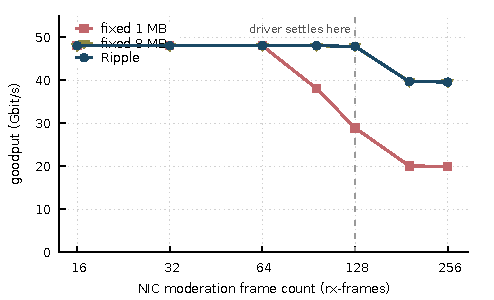
\includegraphics[width=\columnwidth]{figs/fig_frames.pdf}
\caption{Goodput against the NIC's moderation frame count at 48\,Gbps offered,
one core. The cliff is a property of the pair (frames, buffer), not of either
alone. Standard deviations are below 0.05\,Gbps at every point.}
\label{fig:frames}
\end{figure}

\paragraph{Constraint \ref{eq:c1}: the descriptors.}
The collapse past 128 has a different cause. With a 128-entry ring,
\texttt{rx\_out\_of\_buffer} gains 14{,}958 over a run at 128 frames and
1{,}161{,}830 at 192---seventy-seven times as many---and with a 1024-entry ring
it gains nothing at either. The NIC cannot accumulate a moderation window larger
than its ring.

\paragraph{Constraint \ref{eq:c3}: the cache.}
The larger ring is not free. At 128 frames with an 8\,MB buffer, a 128-entry
ring carries 47.86\,Gbps and a 1024-entry ring 36.86: eleven gigabits for the
16\,MB of descriptor pages the larger ring pins in an 18\,MB cache.

\subsection{Moderation is not misbehaving}

Figure~\ref{fig:moderation} gives the ladder. It is tempting to read it as a bug
in the adaptive moderation controller.
It is not. The controller settles immediately on (8\,\textmu s, 128 frames) and
never moves---six runs, zero transitions---so there is no oscillation to damp.
Below the knee it holds throughput equal while taking substantially less CPU:

\begin{figure}[t]
\centering
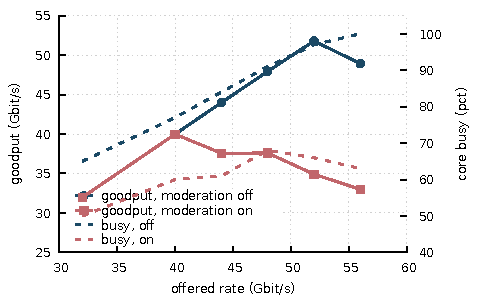
\includegraphics[width=\columnwidth]{figs/fig_moderation.pdf}
\caption{Interrupt moderation, on and off, against offered rate with a fixed
1\,MB buffer. Below 44\,Gbps it holds throughput while saving 15--17 points of
CPU. Above, throughput collapses \emph{with the core idle}: 63\% busy delivering
33\,Gbps at 56 offered. The effect changes sign at the knee.}
\label{fig:moderation}
\end{figure}

\begin{center}
\small
\begin{tabular}{@{}lrrrr@{}}
\toprule
offered & mod.\ off & mod.\ on & busy off & busy on \\
\midrule
32\,G & 31.99 & 31.99 & 65\% & \textbf{50\%} \\
40\,G & 39.98 & 39.98 & 77\% & \textbf{60\%} \\
44\,G & 43.98 & \textbf{37.57} & 84\% & 61\% \\
48\,G & 47.93 & \textbf{37.60} & 91\% & 68\% \\
56\,G & 48.92 & \textbf{32.99} & 100\% & 63\% \\
\bottomrule
\end{tabular}
\end{center}

Below 44\,Gbps moderation is doing exactly its job, saving 15--17 percentage
points of CPU at equal throughput. Above it, the machine drops packets with the
CPU idle---63\% busy while delivering 32.99---which is not exhaustion but a
buffer that cannot hold one window's delivery. The frame count is wrong only
relative to a buffer that was sized without knowledge of it. Disabling
moderation is not a fix; it discards real savings in the regime where the
machine spends most of its time.

\section{The working set is the cache}
\label{sec:workingset}

That constraint (\ref{eq:c3}) is a cache effect rather than a memory-pressure
effect requires evidence beyond the correlation above.

\begin{figure}[t]
\centering
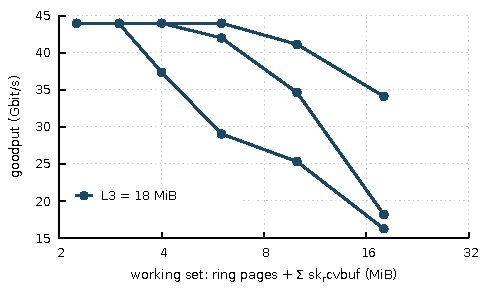
\includegraphics[width=\columnwidth]{figs/fig_workingset.pdf}
\caption{Goodput against working set with the last-level cache partitioned by
Intel CAT. Restricting the receive path to 9 and 4.5\,MiB moves the knee from
10 to 6 to 4\,MiB of working set. Nothing else in the system changes; this is
the causal test that the threshold is the cache.}
\label{fig:workingset}
\end{figure}

\paragraph{The threshold tracks the working set, not the socket count.}
Figure~\ref{fig:workingset} summarises what follows. We vary ring size and
buffer size independently and find the delivered rate
depends only on their sum. A 128-entry ring with a 16\,MB buffer (18\,MiB total)
and a 1024-entry ring with a 4\,MB buffer (20\,MiB total) deliver 33.20 and
33.05\,Gbps respectively. Eight sockets at 2\,MB and one socket at 16\,MB
collapse at the same aggregate. The number of sockets is irrelevant; the sum is
not.

\paragraph{Moving the cache moves the cliff.}
We partition the last-level cache with Intel CAT, restricting the receiving
core to 18, 9, and 4.5\,MiB of ways. The knee moves to 10, 6, and 4\,MiB of
working set respectively---in proportion, and with no other change to the
system. This is the causal test: the threshold is a property of the cache
available to the receive path, not of the amount of memory in use.

\paragraph{Counters agree.}
Hardware counters on the receiving core show last-level load misses rising from
0.0\% of loads at a 6\,MiB working set to 14.3\% at 18\,MiB, with IPC falling
from 1.12 to 1.02 over the same range. The absolute IPC change is small because
the receive path is not compute-bound; what the counters establish is the
mechanism, not its magnitude. The magnitude is in the throughput, and it is
large.

We note one negative result that constrains the interpretation. An earlier
version of this analysis reported a local optimum---a buffer size that was
better than both smaller and larger ones---which would have suggested a tuning
target rather than a bound. It was an artefact: that sweep ran with early
discard enabled, and at small buffers the discard window was continuously
active, which manufactured the left-hand side of the curve. With discard
disabled the relationship is monotone from 512\,KB to 18\,MB. There is no
optimum to find; there is only a ceiling not to cross, which is why \sys bounds
rather than targets.

\subsection{Why a larger buffer costs}

That a working set exceeding the cache costs throughput is unsurprising. Less
obvious is \emph{which} traffic pays. We separated the producer (NAPI, building
and queueing \texttt{skb}s) from the consumer (\texttt{recvmsg}, copying out)
onto different cores and varied only the cache level they share, sweeping the
buffer from 512\,KB to 18\,MB in each arrangement:

\begin{center}
\small
\begin{tabular}{@{}lr@{}}
\toprule
cache shared by producer and consumer & 512\,KB $\to$ 18\,MB ratio \\
\midrule
L2 and L3 (same core) & \textbf{0.40} \\
L3 only (same socket) & 0.61 \\
none (different sockets) & \textbf{0.94} \\
\bottomrule
\end{tabular}
\end{center}

With no shared cache, buffer size is almost irrelevant. The cost of a large
buffer is therefore not the memory it occupies but the \emph{hand-off} it
breaks: data queued in a small buffer is still resident when the consumer
reaches it, and data queued in a large one has been evicted. This is why
growth must stop at the measured demand rather than continue while a global
limit still permits it---the penalty begins well before the limit is reached.

\paragraph{Consequence for sizing.} The quantity to bound is
$\texttt{ring bytes} + \sum \texttt{sk\_rcvbuf}$ against the last-level cache.
A per-socket limit cannot express this: 4\,MB is entirely safe for one socket
and ruinous as the eighth. Any mechanism that sizes buffers must therefore have
a global term.

\section{Two workloads, one machine}

We now show the two constraints pull apart on ordinary workloads. Both run on
the same kernel with the same settings and the driver's moderation at its
default; only the traffic differs.

\begin{description}
\itemsep0em
\item[W1] one socket receiving 56\,Gbps. Burst-dominated: each moderation window
delivers about 1.15\,MB to one queue.
\item[W2] eight sockets receiving 7\,Gbps each. Working-set-dominated: no single
queue is stressed, but every buffer counts against the cache.
\end{description}

\begin{table}[t]
\centering
\small
\begin{tabular}{@{}lrrrr@{}}
\toprule
& \multicolumn{2}{c}{W1: one socket} & \multicolumn{2}{c}{W2: eight sockets} \\
\cmidrule(lr){2-3}\cmidrule(lr){4-5}
configuration & Gb/s & loss & Gb/s & loss \\
\midrule
\multicolumn{5}{@{}l}{\emph{moderation on, the driver default}} \\
\quad fixed 1\,MB & 35.4 & 36.9 & 55.7 & 0.6 \\
\quad fixed 1\,MB + shed & 54.2 & 3.1 & 55.8 & 0.3 \\
\quad fixed 8\,MB & 55.6 & 0.8 & 22.9 & 59.1 \\
\quad fixed 8\,MB + shed & 55.5 & 1.0 & 29.5 & 47.3 \\
\quad \sys & 55.4 & 1.0 & 55.6 & 0.7 \\
\quad \sys + shed & 55.6 & 0.7 & 55.8 & 0.4 \\
\midrule
\multicolumn{5}{@{}l}{\emph{moderation off}} \\
\quad fixed 1\,MB & 48.2 & 14.0 & 50.3 & 10.1 \\
\quad fixed 1\,MB + shed & 52.7 & 5.9 & 52.3 & 6.6 \\
\quad fixed 8\,MB & 40.3 & 28.1 & 19.8 & 64.7 \\
\quad fixed 8\,MB + shed & 46.0 & 17.9 & 25.3 & 54.7 \\
\quad \sys & 45.4 & 19.0 & 46.2 & 17.5 \\
\quad \sys + shed & 48.9 & 12.8 & 51.5 & 8.0 \\
\bottomrule
\end{tabular}
\caption{Both workloads on one kernel and one setting, $n=10$.
Loss is what the sender offered and the receiver did not deliver;
goodput alone does not distinguish carrying a load from discarding
much of it. Each fixed buffer loses one workload badly. A small one
with driver-side discard carries both under either moderation
setting; a large one with the same discard still does not.}
\label{tab:nostatic}
\end{table}


\begin{figure}[t]
\centering
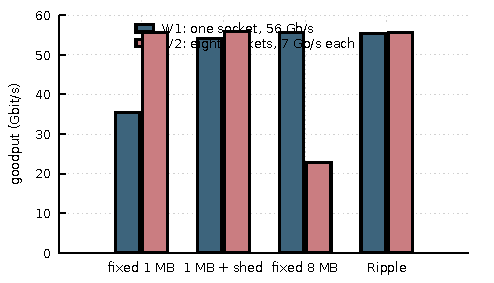
\includegraphics[width=\columnwidth]{figs/fig_workloads.pdf}
\caption{The same kernel and the same settings on two ordinary workloads. Each
fixed buffer wins one column and loses the other by 37--58\%. A small buffer
with driver-side discard wins both; a large one with the same discard still
loses W2, because what fails there is the capacity rather than the work.}
\label{fig:workloads}
\end{figure}

Table~\ref{tab:nostatic} and Figure~\ref{fig:workloads} give the result. A
1\,MB buffer cannot hold a moderation window and drops 37\% of W1; eight 8\,MB
buffers are three times the cache and drop 58\% of W2. Neither is a
pathological setting---each is the right answer for the other workload---and an
operator who has tuned for one will be running the other within the hour.

Two further rows decide the shape of the rest of the paper. Adding the discard
of \S\ref{sec:d-burst} to the 1\,MB buffer carries both workloads---54.2 and 55.8,
at 3.1\% and 0.3\% loss---and does so under either moderation setting. Adding
the same discard to the 8\,MB buffer does not rescue W2: 22.9 becomes 29.5 and
stops, still losing 47\% of what was offered.

The asymmetry is the whole design. A buffer too small for a burst can be
repaired by not doing the work. A buffer too large for the cache cannot be
repaired at all, because what thrashes is the capacity and discarding removes
only work. One of the two failures admits a cheap fix after the fact; the other
must be prevented before the buffer exists.

We stress that these are not adversarial workloads. A single high-rate flow and
a handful of moderate ones are both routine.

\section{Design}
\label{sec:design}

\sys is two mechanisms and no controller. This section takes the five problems
of \S\ref{sec:problems} in order (Table~\ref{tab:map}) and says what addresses
each, including the one we tried first and discarded.

\begin{table}[t]
\centering
\small
\begin{tabular}{@{}llp{3.1cm}@{}}
\toprule
 & problem & addressed by \\
\midrule
P1 & burst of unknown size & \S\ref{sec:d-burst}: discard, not growth \\
P2 & the sum is global & \S\ref{sec:d-cap}: cache-derived cap \\
P3 & larger is worse past the ceiling & \S\ref{sec:d-burst}, and why we do not size \\
P4 & work spent before the drop & \S\ref{sec:d-place}: discard in the driver \\
P5 & per socket vs per queue & \S\ref{sec:d-select}: select by L4 type \\
\bottomrule
\end{tabular}
\caption{Each problem and the part of the design that answers it.}
\label{tab:map}
\end{table}

\subsection{P1 and P3: absorb the burst by not doing the work}
\label{sec:d-burst}

P1 asks for a buffer large enough to hold one moderation window. P3 says a
larger buffer is harmful past the point where the consumer falls behind. Taken
together they rule out the obvious answer, because the two are not separate
regimes: the same socket crosses from one to the other as its offered rate
rises, and a mechanism that grows the buffer for P1 is still growing it when P3
applies.

\sys therefore does not grow the buffer. When the socket queue is full, the
driver stops delivering UDP completions for a short window, discarding them
before an \texttt{skb} exists. The burst is absorbed by shrinking it rather than
by making room for it, and the buffer stays small enough that what is queued is
still resident when the consumer arrives.

\paragraph{The window is fixed at 50\,\textmu s.} We swept it from 25 to
1600\,\textmu s and found the response asymmetric: too short costs 7\%, too long
costs 67\%, and 1600\,\textmu s is worse under a load transition than no window
at all. An adaptive controller is possible; the oracle's advantage over a fixed
50\,\textmu s is 1.6\%, which is less than the cost of searching for it.

\paragraph{Why not size the buffer.} We built the adaptive sizer the problem
statement suggests---TCP's rule with the interval between the receive queue
filling and emptying standing in for the RTT---and report it in
\S\ref{sec:sizing}. It works, and it is not better than this. The reason is P3:
the estimate it converges on is ``as much buffer as this socket can use'', and
the measurement says the quantity worth minimising is how much data sits between
producer and consumer.

\subsection{P2: a cap derived from the cache}
\label{sec:d-cap}

\sys reads the last-level cache size from the kernel's cache topology at boot
and takes a configurable fraction of it, one half by default, as an allowance. A
socket's whole buffer is charged against the total once, on the first packet it
receives, and returned when the socket is destroyed.

\paragraph{A bound, not a target.} The allowance does not look for a good size.
It prevents individually reasonable sizes from summing to a bad one, which is
exactly what P2 says a per-socket limit cannot do. Within the allowance, what
the application or the operator asked for stands.

This is a weaker mechanism than a controller, and deliberately so.
\S\ref{sec:workingset} establishes a claim about the sum and says nothing about
where within the bound a given socket should sit. A cap is the mechanism that
claim licenses.

\paragraph{What the implemented cap does and does not do.} It refuses any
\emph{increase} that would take the total past the allowance. It does not
currently refuse the buffer a socket starts with: a machine configured with an
8\,MB \texttt{rmem\_default} and eight sockets is charged 64\,MB and permitted
it. The measurement in Table~\ref{tab:nostatic} showing that discarding fails to
rescue eight 8\,MB buffers is therefore evidence that such a cap is
\emph{needed}, not that ours enforces it. Clamping the default---as against an
explicit \texttt{SO\_RCVBUF}, which we argue below should be honoured---is the
obvious extension; it requires deciding what a socket gets when the allowance is
already spent, and we have not measured our way to an answer.

\paragraph{Capacity, not occupancy.} The allowance bounds granted capacity
rather than queued bytes. Bounding queued bytes is the natural first attempt and
does not work: while the consumer keeps up the queues sit nearly empty---0.36\,MB
held against 8\,MB of capacity in one measurement---so the bound does not bite
until the queues have grown deep, by which point the buffers behind them are far
too large. Occupancy follows capacity, not the reverse.

\paragraph{All of it is charged.} The whole buffer, not the part above some
default. Counting only the excess leaves the baseline invisible, and the
baseline is not small when there are many sockets: eight at a 1\,MB default are
8\,MB of a 9\,MB allowance before anything else happens. An earlier version
charged only what it had itself handed out, and eight sockets reached 17.8\,MB
against a 9\,MB allowance.

\paragraph{Sockets that set \texttt{SO\_RCVBUF}.} An application that names a
size still receives it; overriding an explicit request would break a long
standing expectation, and in isolation the request is rarely the problem. \sys
charges such a socket for what it holds so that everyone else stops compounding
it: 64\,MB is entirely safe until it is the eighth one.

\paragraph{Why the fraction is an operator setting.} We would prefer the
allowance to be fully derived, and it nearly is---the cache size comes from the
kernel's own topology, so it follows the hardware. What the kernel cannot see
from the socket layer is how much of that cache is already committed. The
dominant unseen term is the NIC's descriptor pages, 16\,MB for a 1024-entry ring
on our hardware, which the driver allocates and never surfaces in a form the
socket layer can query. A fully automatic version is possible---the driver knows
the ring size and the descriptor format---but it would put the mechanism behind
a per-driver change, and one number per machine is a considerably better
interface than one number per socket.

\subsection{P4: discard where the work has not yet been done}
\label{sec:d-place}

Placement is the whole of P4. A drop at the socket happens after the packet has
cost descriptor processing, an \texttt{skb} allocation, GRO, and a route lookup;
a drop at the completion queue costs a comparison. \sys marks the receive queue
on which a socket drop occurred, and for the window the driver discards matching
completions in \texttt{mlx5e\_handle\_rx\_cqe()} before any of that work
happens.

\paragraph{Take the queue from the packet, not the socket.} The queue to hold
back is the one that delivered the packet which could not be queued. Reading it
from the socket instead, via \texttt{sk\_rx\_queue\_get()}, is wrong in a way
that appears only with more than one queue: that field is maintained for
connected sockets, and an unconnected socket---the many-senders case UDP exists
for---reads back $-1$, which a fallback turns into queue zero. Every such socket
then throttles queue zero regardless of which queue was drowning.

\subsection{P5: discard selectively}
\label{sec:d-select}

The completion descriptor carries the L4 header type, so the discard can be
restricted to UDP. This is what allocation structurally cannot do. Buffers are
per socket while the queue is shared, so when TCP and UDP contend for one queue,
no setting of the UDP socket's buffer gives TCP more of it; what TCP is short of
is service, not space. Declining to build \texttt{skb}s for one protocol leaves
the core free for the other, and \S\ref{sec:evalproto} measures the result.


\section{Sizing the buffer: a negative result}
\label{sec:sizing}

Before arriving at a cap and a discard we built the thing the problem statement
suggests: a controller that sizes each buffer to what its traffic needs. It
works, in the sense that it reaches parity with the better fixed buffer on both
workloads without being told which workload it is running. It is nonetheless not
the right mechanism, and the reason is worth more than the mechanism would have
been.

\subsection{The construction}

TCP's receive-side rule is $\rcvbuf = 2 \times (\text{bytes received in one
RTT})$: the RTT delimits one turn of the consumer, and the factor of two leaves
room for the next turn's arrivals while the current one is consumed. UDP has no
RTT, which is the usual reason given for the absence of UDP autotuning.

The RTT's role, though, is only to delimit a period over which demand can be
measured, and the receive queue supplies one: the interval from its rising above
half full to its falling below an eighth. Over that interval the queue's peak is
what arrived while the consumer worked through what it already had---which, when
the NIC is batching, is one moderation window's delivery. Sizing to twice it
reproduces TCP's rule with a clock UDP can read, and lands on
$\rxframes \times \texttt{pkt}$ without consulting the driver.

Two properties fall out. A socket whose consumer cannot keep up never sees its
queue empty, so it never closes an interval, never produces a target, and never
grows---the case where more buffer cannot help excludes itself, with no separate
test. And a cycle must be closed by \emph{both} halves: detecting only the drain
is insufficient, because the enqueue path runs on every arrival and a socket
whose queue is already empty would close a cycle on each packet, with a peak of
one packet, overwriting a correct target with nothing.

\subsection{Why it is not the answer}

Table~\ref{tab:nostatic} places it against the alternatives. It matches the
better fixed buffer on both workloads. It does not beat a fixed 1\,MB buffer
combined with the discard of \S\ref{sec:shed}, which matches it below the
receiving core's saturation point and exceeds it by 4--6\% above
(Figure~\ref{fig:shedmarg}).

The reason is the measurement that motivated the sizer in the first place. Past
the point where arrivals outpace the consumer, the queue is full whatever its
capacity, and the extra capacity only lengthens the time data waits before
copy-out---by which time, per \S\ref{sec:workingset}, it has been evicted.
Sizing up is the wrong response to overload, and an adaptive sizer is a machine
for sizing up.

There is a second, sharper way to see this. The demand figure is the queue's
peak occupancy, and occupancy is bounded by \rcvbuf. A larger buffer therefore
permits a deeper peak, which raises the estimate, which grows the buffer again;
the loop is stopped by the allowance rather than by need, and we measured it
reaching 9.4\,MB on a socket that performed better at 1. TCP does not have this
problem because \texttt{tcp\_rcv\_space\_adjust()} counts bytes \emph{copied to
the application}, which buffer size cannot inflate. Counting bytes released to
the consumer over the same interval would be the faithful translation and would
remove the inflation.

We did not pursue it, because by then the conclusion no longer depended on the
estimator. Even a perfectly calibrated sizer converges on ``as much buffer as
this socket can use'', and the measurement says the quantity worth minimising
is how much data sits between the producer and the consumer. The right target is
small, and a mechanism whose whole purpose is to find how large it may safely be
is aimed the wrong way.

\subsection{What the exercise established}

Two things, both of which the final design rests on.

That \emph{discarding cannot substitute for a cap.} Eight sockets at 8\,MB reach
22.7\,Gbps, and 29.4 with discarding enabled---an improvement, and still half of
the 55.8 the same eight reach at 1\,MB, still losing 47\% of what was offered.
Removing work does not remove capacity. Whatever else is done, something has to
bound what the buffers sum to.

And that \emph{a cap is all the sizing that is needed.} Between the cap and the
discard, the remaining freedom---where within the bound a given socket sits---is
worth at most the 0.2\,Gbps by which the sizer leads the fixed buffer below the
ceiling, and costs 4--6\% above it.


\section{Implementation}

\sys is implemented in Linux 6.18. The allowance is 90 lines in
\texttt{net/ipv4/udp.c} plus two atomic fields in \texttt{struct udp\_sock}; the
discard is 40 lines in the mlx5 receive path plus a per-queue timestamp array.
Both are controlled by \texttt{sysctl}s and default to off, so an unconfigured
kernel behaves exactly as upstream---the charging function returns its argument
unchanged on the first test.

\paragraph{Lock-free operation.} The charge runs in
\texttt{\_\_udp\_enqueue\_schedule\_skb()} \emph{before} it takes the receive
queue lock, and a socket with many senders is delivered from as many queues as
those senders hash to. The first charge is therefore claimed with an
\texttt{atomic\_cmpxchg} against zero, so exactly one caller pays it and the
rest observe it done. Plain read-modify-write loses updates, and a lost update
here is not self-correcting: \texttt{udp\_destruct\_common()} returns the
per-socket figure, so anything the global counter gained and the per-socket
counter did not is never given back, and enough of them exhaust the allowance
permanently.

\paragraph{Cost.} On the enqueue fast path \sys adds one atomic read in the
common case---the charge fires once per socket lifetime---and the discard check
is a read of a per-queue timestamp and, on the rare non-zero path, a comparison
against a monotonic clock. We measure no throughput difference with either
mechanism enabled but inactive.

\section{Evaluation}
\label{sec:eval}

\paragraph{Setup.} Two machines, Xeon Silver 4310 (Ice Lake-SP, 12 cores per
socket, 48\,KB L1d, 1.25\,MB L2 per core, 18\,MB L3 per socket), NVIDIA
ConnectX-5 100\,GbE, MTU 9000, Ubuntu 20.04, Linux 6.18.53. Unless stated, the
receiver uses one queue with its interrupt pinned to the same core as the
consumer, a 128-entry ring, the performance governor, and the driver's default
adaptive moderation. This is a genuinely single-core configuration: RPS is off
and we verify the interrupt lands on the intended core.

\paragraph{Methodology.} We drive the receiver with a purpose-built generator
that paces on a byte budget rather than a timer. Standard tools pace with
\texttt{clock\_nanosleep}, whose wake-up granularity produces bursts that
fabricate loss below the true ceiling; we spent considerable effort on
mechanisms that turned out to be artefacts of this before instrumenting the
tool. Goodput is measured at the receiving application. Kernel counters cannot
substitute: interface \texttt{rx\_bytes} counts what arrived on the wire
including what was then dropped, and \texttt{Udp:InDatagrams} counts GRO
super-\texttt{skb}s rather than datagrams, understating delivery by the merge
factor. Every point is five runs; we discard runs where the sender fell short of
its target.

\subsection{Does it carry both workloads?}
\label{sec:evalworkloads}

Table~\ref{tab:nostatic} is the primary result. \sys---a 1\,MB buffer inside
the cap, with the discard---delivers 54.2 and 55.8\,Gbps where the better fixed
buffer alone delivers 35.4 and 22.9, improving the worst case by 1.53$\times$
over the best single fixed choice.

We also give the adaptive sizer, because the comparison is close and reporting
only the favourable half would be misleading. At this operating point sizing is
marginally ahead: 55.4 and 55.6, and 55.6 and 55.8 with the discard added, which
is 2.6\% better in the worst case than the fixed buffer with discard. It is
behind by 7\% with moderation disabled (48.9 against 52.3) and by 4--6\% past
the ceiling (\S\ref{sec:evalshed}). Nothing dominates; the fixed buffer with
discard is the configuration that is never far from the best, and it is the one
that needs no per-socket state.

The rows that separate the two \emph{mechanisms}, as opposed to the two
policies, are the 8\,MB pair. Discard added to a large buffer rescues only the
workload that was never in difficulty. A cap is therefore not an optimisation on
top of the discard; it is what keeps the discard's job doable.

\subsection{Does the cap matter?}

The cap only acts when buffers would otherwise sum past the cache, so it is
invisible on a machine that was going to be fine. Where it acts, it is not a
refinement. With eight sockets free to take what they ask for and no allowance,
throughput falls to 16.5\,Gbps against 47.9 for the stock configuration; with
the allowance, 47.4. The same effect is what separates the two discard rows of
Table~\ref{tab:nostatic}: discarding cannot undo capacity already granted, so
the only point at which the eight-socket case can be saved is before the
granting.

\subsection{Many senders, one socket}

The case UDP has and TCP does not is many senders writing to one socket, and we
find the effect conditional on something we had not expected to matter: whether
the senders use segmentation offload (Figure~\ref{fig:fanin}).

With GSO the merge factor is 6.4 at sixty-four flows exactly as at one. The
reason is that GSO lays one flow's seven packets contiguously on the wire, so
GRO never has to hold several flows open at once, and its fixed bucket count is
never tested. Without GSO the flows interleave, the merge factor falls from 6.6
to 1.0 across the same range, and the CPU cost of a fixed 30\,Gbps rises from
46\% to 60\% busy. With two sending cores it breaks the ceiling: at 68\,Gbps
offered, two flows deliver 60.7 and sixty-four deliver 38.7, and the sixty-four
figure falls further as the offered rate rises.

This is a limit of GRO's bucket count, not of buffer sizing, and neither
mechanism here addresses it. We report it as a boundary of the contribution, and
note that the condition under which it bites---high aggregate rate from many
senders, none of them using offload---is one an operator can do something about.

\begin{figure}[t]
\centering
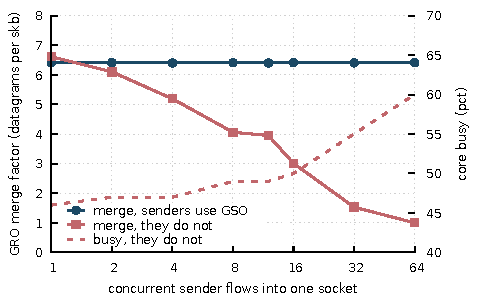
\includegraphics[width=\columnwidth]{figs/fig_fanin.pdf}
\caption{Many senders into one socket, 30\,Gbps aggregate. Coalescing survives
sixty-four flows when the senders use segmentation offload and collapses without
it, because offload is what keeps one flow's packets adjacent on the wire.}
\label{fig:fanin}
\end{figure}

\subsection{Where allocation stops helping}
\label{sec:evalshed}

Everything above allocates buffer, and allocation has a ceiling: once the
receiving core is saturated, no distribution of buffer changes how much work
there is. Figure~\ref{fig:shedmarg} extends the offered rate past that point
with and without the driver-level shedding of \S\ref{sec:d-burst}.

Table~\ref{tab:shedmarg} gives the ladder. Two things are visible, and the
second is uncomfortable. Sizing carries the load
up to the ceiling---at 48 and 56\,Gbps, \sys and \sys with shedding are within
0.5\,Gbps of each other, so the discard window is doing nothing---and past it
only shedding changes anything: at 72 and 80\,Gbps \sys alone turns over to 54.2
and 54.9 while shedding holds 58.1 and 58.6.

The uncomfortable result is the fourth arm. A \emph{fixed} 1\,MB buffer with
shedding reaches 62.7, 61.4, and 60.9 at 64, 72, and 80\,Gbps---ahead of \sys
with shedding at every one of them, and by 4--6\%. The only difference between
those two arms is buffer size, so this is the cache hand-off of
\S\ref{sec:workingset} appearing from the other side: past the ceiling the queue
is full whatever its capacity, and the larger capacity only means more data
resident and evicted before the consumer reaches it. Sizing up is the wrong
response to overload, and \sys sizes up because its demand estimate is taken
from queue occupancy, which its own growth inflates.

We take this as a limitation rather than a refutation, for two reasons that the
evaluation supports and one that it does not. It supports, first, that the two
arms are equal below the ceiling, which is where a receiver is expected to
operate and where shedding discards packets a correctly sized buffer delivers;
and second, that shedding is a per-driver change while sizing is not. What it
does not yet settle is the multi-socket case, where the failure mode is the
buffers' own cache footprint rather than the arrival rate, and where shedding
has no mechanism to help: it removes work, not capacity. We return to this in
\S\ref{sec:evalworkloads}.

\begin{figure}[t]
\centering
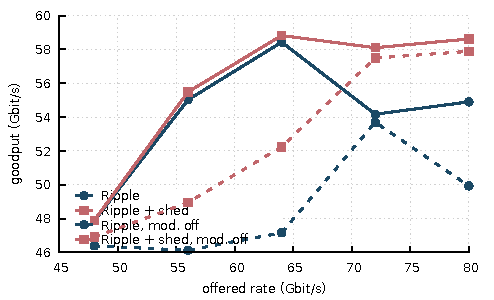
\includegraphics[width=\columnwidth]{figs/fig_shedmarg.pdf}
\caption{Past the core's ceiling, sizing alone cannot help: the queue is full at
every size. Shedding at the driver removes the work instead, and is the only
lever with any effect in that regime.}
\label{fig:shedmarg}
\end{figure}

\begin{table}[t]
\centering
\small
\begin{tabular}{@{}lrrrrr@{}}
\toprule
offered (Gb/s) & 48 & 56 & 64 & 72 & 80 \\
\midrule
\multicolumn{6}{@{}l}{\emph{moderation on (the default)}} \\
\quad \sys & 47.9 & 55.0 & 58.4 & 54.2 & 54.9 \\
\quad \sys + shed & 47.9 & 55.5 & 58.8 & 58.1 & 58.6 \\
\quad fixed 1\,MB & 33.3 & 34.0 & 34.4 & 36.0 & 38.7 \\
\quad fixed 1\,MB + shed & 47.5 & 54.7 & 62.7 & 61.4 & 60.9 \\
\midrule
\multicolumn{6}{@{}l}{\emph{moderation off}} \\
\quad \sys & 46.4 & 46.1 & 47.2 & 53.7 & 49.9 \\
\quad \sys + shed & 46.9 & 49.0 & 52.2 & 57.5 & 57.9 \\
\quad fixed 1\,MB & 47.9 & 48.1 & 49.5 & 55.1 & 52.4 \\
\quad fixed 1\,MB + shed & 48.0 & 52.7 & 55.8 & 61.5 & 61.7 \\
\bottomrule
\end{tabular}
\caption{Goodput past the ceiling, $n=5$ per point. Sizing carries the
load up to the ceiling; only shedding changes anything beyond it.}
\label{tab:shedmarg}
\end{table}


\subsection{Protocol isolation under a shared queue}
\label{sec:evalproto}

A socket buffer is per socket; the bottleneck under study is per queue. When TCP
and UDP share a receive queue, no amount of UDP buffer tuning gives TCP its
share, because the resource TCP is short of is not buffer. Shedding is
selective---the completion descriptor carries the L4 type---so it can make room
for one protocol by discarding another's packets before they cost anything.

Table~\ref{tab:protiso} gives a UDP flow at 64\,Gbps and a TCP flow sharing one
queue and one core. Discarding raises the aggregate by 10--12\% in both buffer
configurations, 63.3 to 69.7 with a fixed buffer and 65.0 to 73.0 with \sys. We
claim the aggregate and not the split: which protocol collects the gain depends
on the buffer, TCP with a fixed 1\,MB (35.9 to 41.3) and UDP with \sys (29.6 to
40.5). The mechanism makes room; it does not decide who takes it.

\begin{table}[t]
\centering
\small
\begin{tabular}{@{}lrrr@{}}
\toprule
configuration & UDP & TCP & total \\
\midrule
fixed 1\,MB & 27.4 & 35.9 & 63.2 \\
fixed 1\,MB + shed & 28.3 & 41.3 & 69.7 \\
\sys & 29.6 & 35.4 & 65.0 \\
\sys + shed & 40.5 & 32.5 & 73.0 \\
\bottomrule
\end{tabular}
\caption{A UDP flow and a TCP flow sharing one receive queue and one
core, $n=5$. Discarding raises the aggregate by 10--12 percent in both
buffer configurations; which protocol collects the gain depends on
the buffer, so we claim the total and not the split.}
\label{tab:protiso}
\end{table}


\subsection{When the application does not ask for coalescing}

Our measurements so far have the receiving application set \texttt{UDP\_GRO}, so
the kernel hands over coalesced buffers. An application that does not set it
gets \texttt{udp\_rcv\_segment()}, which splits the coalesced buffer back into
datagrams---undoing work the stack just did---and the per-\texttt{skb} cost
rises accordingly, lowering the ceiling. The mechanisms are indifferent to this:
\sys reads only the queue, and shedding reads only the completion descriptor.
The \emph{operating points} are not.

Table~\ref{tab:groleverson} and Table~\ref{tab:groleversoff} give the ladders.
Measured at 56\,Gbps with moderation at its default, a fixed 1\,MB buffer
delivers 36.7 with coalescing requested and 30.0 without; adding discard gives
54.2 and 47.5, and \sys gives 55.3. Re-segmentation costs about 7\,Gbps of
ceiling and raises the CPU per byte---the discard arm runs at 94\% busy without
coalescing against 85\% with it---but neither lever stops working. What changes
is which one pays: once the core saturates, only removing work helps, so the
gap between \sys and discard narrows as the per-packet cost rises.

\begin{table}[t]
\centering
\small
\begin{tabular}{@{}lrrrrr@{}}
\toprule
offered (Gb/s) & 24 & 32 & 40 & 48 & 56 \\
\midrule
\multicolumn{6}{@{}l}{\emph{application sets UDP\_GRO}} \\
\quad fixed 1\,MB & 24.0 & 32.0 & 40.0 & 48.0 & 36.7 \\
\quad + shed & 24.0 & 32.0 & 40.0 & 47.9 & 54.2 \\
\quad \sys & 24.0 & 32.0 & 40.0 & 47.9 & 55.3 \\
\midrule
\multicolumn{6}{@{}l}{\emph{it does not; the stack re-segments}} \\
\quad fixed 1\,MB & 24.0 & 32.0 & 40.0 & 32.9 & 30.0 \\
\quad + shed & 24.0 & 32.0 & 40.0 & 46.4 & 47.5 \\
\quad \sys & 24.0 & 32.0 & 40.0 & 45.9 & 46.9 \\
\bottomrule
\end{tabular}
\caption{Goodput with moderation on. Re-segmentation raises the
per-packet cost and lowers the ceiling, which changes which lever pays.}
\label{tab:groleverson}
\end{table}

\begin{table}[t]
\centering
\small
\begin{tabular}{@{}lrrrrr@{}}
\toprule
offered (Gb/s) & 24 & 32 & 40 & 48 & 56 \\
\midrule
\multicolumn{6}{@{}l}{\emph{application sets UDP\_GRO}} \\
\quad fixed 1\,MB & 24.0 & 32.0 & 40.0 & 47.9 & 48.0 \\
\quad + shed & 24.0 & 32.0 & 40.0 & 48.0 & 52.6 \\
\quad \sys & 24.0 & 32.0 & 40.0 & 45.2 & 45.7 \\
\midrule
\multicolumn{6}{@{}l}{\emph{it does not; the stack re-segments}} \\
\quad fixed 1\,MB & 24.0 & 32.0 & 40.0 & 43.2 & 35.4 \\
\quad + shed & 24.0 & 32.0 & 40.0 & 46.3 & 44.0 \\
\quad \sys & 24.0 & 32.0 & 40.0 & 40.4 & 34.6 \\
\bottomrule
\end{tabular}
\caption{Goodput with moderation off. Re-segmentation raises the
per-packet cost and lowers the ceiling, which changes which lever pays.}
\label{tab:groleversoff}
\end{table}



\subsection{More than one receive queue}

A single queue is the configuration in which the receive path's costs are
easiest to attribute, but it is not the common deployment. With $n$ queues the
descriptor footprint is $n$ times larger---the term in constraint (\ref{eq:c3})
neither mechanism can see---and the flow-to-core assignment becomes RSS's choice
rather than the application's, which matters because producer and consumer
sharing a cache is worth up to 2.5$\times$ (\S\ref{sec:workingset}).

We cannot measure this on our hardware, and the reason is worth stating
precisely rather than leaving as an omission. One core carries about 55\,Gbps.
Two therefore saturate a 100\,GbE link before either is the bottleneck, and with
four the link binds so far ahead of the receive path that every configuration we
tested returned the offered rate at a quarter of one core's capacity: 48.00\,Gbps
in all six arms, 25\% busy. A receive-CPU-bound multi-queue experiment needs
either a faster link or a slower core than we have.

What can be said without measuring is the direction. The descriptor term grows
with the queue count while the cache does not, so the allowance has strictly
less room to distribute---at a 1024-entry ring, eight queues would pin more than
the whole cache in descriptor pages alone. This makes the cap more binding with
more queues, not less, which is the opposite of the usual assumption that
spreading work across cores relieves pressure. Verifying it requires hardware
where the receive path can still be the bottleneck at eight queues.

\subsection{Sensitivity to moderation}

The discard is armed by a socket drop, so it should follow the moderation
setting without being told it. Sweeping \rxframes at 48\,Gbps with a 1\,MB
buffer and the discard enabled holds throughput flat across 16 to 128 frames,
where the same buffer without it falls from 47.98 to 28.93. The mechanism needs
no knowledge of the frame count because it responds to the consequence of the
frame count.

The sizer, for comparison, also tracked it---47.98, 47.98, 47.99, 47.98, 47.89
across the same sweep. Both mechanisms follow the setting; only one of them
needs a per-socket state machine to do so.

\section{Discussion and limitations}

\paragraph{When there is nothing to absorb.} With moderation disabled, no large
bursts arrive. The discard still pays---it is armed by drops, and drops still
happen at overload---but there is nothing for a buffer to absorb, and the sizer
we discarded was measurably worse than a fixed 1\,MB buffer in that regime
(45.7 against 48.1, and 45.0 against 49.1). This is the clearest statement of
why sizing is not the mechanism: in the case where adapting has nothing to do,
adapting still costs.

\paragraph{Fairness is argued, not shown.} We adopt additive increase for its
convergence properties, but could not construct a workload on this hardware
where multiplicative increase measurably harms fairness: with several sockets
sharing one core, none obtains enough rate to run away, and Jain's index over
goodput remained above 0.999 in every arm. The unfairness we did observe was
temporal---a socket that grew and then went quiet denying a newcomer---which
reclamation addresses directly.

\paragraph{Deploying this.} Both mechanisms default to off, and with the knobs
off the kernel's behaviour is identical to upstream---the sizing function
returns its argument unchanged on the first test. An operator can therefore
enable sizing on a fraction of a fleet and compare, which is how we would expect
a change of this kind to be adopted. The allowance fraction is the one value
that has to be chosen, and the consequence of choosing it too high is bounded:
the machine behaves as it does today with a large static buffer.

\paragraph{What we would want next.} The sizing responds to the consumer it has,
so a socket whose application is slow gets no more buffer, which is correct.
What it cannot do is tell the application that it is slow. A receiver that could
see ``your buffer is not the constraint, your \texttt{recvmsg} loop is'' would
be more useful than one that silently stops growing, and the information exists
at the point where \sys declines to grow.

\paragraph{One NIC, one cache topology.} All measurements are on ConnectX-5 with
an 18\,MB last-level cache. The cache size is read at boot, so the allowance
follows different hardware by construction, but we have not verified the cliff's
position on a different cache organisation. The descriptor-page footprint is
NIC-specific: our figure of 16\,MB for a 1024-entry ring follows from the
multi-packet WQE format and would differ elsewhere.

\paragraph{The driver hook.} The shedding of \S\ref{sec:d-burst} requires a change
in each driver, which is a real deployment cost. The buffer sizing does not, and
covers the regime below the core's ceiling; the two divide cleanly, and an
operator who cannot patch a driver still gets the primary result.

\section{Related work}

\paragraph{Receive buffer autotuning.} TCP's dynamic right-sizing is the obvious
precedent, and we report in \S\ref{sec:sizing} what happened when we transplanted
it: it works and it is not what the problem needed. We are not aware of prior
work that supplies a demand-measurement clock for a protocol without
acknowledgements, and we think the construction is sound even though we do not
use it---the interval between a receive queue filling and emptying is a
consumer turn in exactly the sense an RTT is.

\paragraph{Cache-aware networking.} Work on DDIO has shown the effective cache
available to a NIC is smaller than nominal and subject to conflict misses.
That line of work reallocates cache; ours takes the cache as given and sizes the
software's demand to fit it. The two compose: a system that recovers effective
capacity enlarges the allowance \sys distributes.

\paragraph{Active queue management.} CoDel and its descendants decide when to
drop based on how long packets have been queued. Our shedding is adjacent but
differs in placement and in purpose: it discards at the driver so that the
dropped packet costs no CPU, and it is protocol-selective because the bottleneck
is a shared queue rather than a per-socket buffer.

\paragraph{Buffer bloat.} A long line of work argues that large network buffers
harm latency by allowing standing queues. Our argument is different in kind and
happens to point the same way: we find large buffers harm \emph{throughput}, on
the receive side, through the cache rather than through queueing delay, and the
harm appears well before the buffer is full. The two arguments compose---both
conclude that a buffer should be sized to what is needed rather than to what is
affordable---but neither implies the other, and the mechanism we measure would
be invisible to a latency-based analysis.

\paragraph{Kernel-bypass receivers.} Systems that move the receive path to user
space avoid the socket buffer entirely and manage their own memory, which makes
the sizing question explicit rather than absent. The constraint we identify does
not go away there: a user-space receiver still has a ring, still has a cache,
and still has to decide how much to buffer. What changes is that one component
is in a position to see all three quantities. That such systems must solve this
by hand is, we think, evidence that it is a real problem rather than an artefact
of the socket API.

\paragraph{Interrupt moderation.} Adaptive moderation has a long history, and
our results are not a criticism of it: it saves 15--17 points of CPU below the
knee. Our finding is that its output is an input to a sizing decision made
elsewhere, by a party that cannot see it.

\section{Conclusion}

The UDP receive buffer is asked of parties who cannot compute it. Its correct
value depends on a driver setting the application cannot see and on a cache
total no single socket can observe, and the two requirements move in opposite
directions: too small for a moderation window costs 37\% of one workload, too
large for the cache costs 58\% of another.

Our first answer was to compute it for them, and the interesting result is that
this is not what the problem needs. A buffer too small for a burst can be
repaired by not doing the work, and a small buffer with a driver-side discard
carries both workloads. A buffer too large for the cache cannot be repaired at
all, because it is the capacity that thrashes and discarding removes only work.
What is left is a cap and a discard---two mechanisms, no controller---and the
recommendation they imply is the opposite of the one we set out to justify:
keep the buffer small, bound what the buffers may sum to by the cache, and stop
building the ones the consumer will not reach.

\end{document}
